\documentclass[border=8pt]{standalone}
\usepackage{amsmath,amssymb,bm}
\usepackage{xcolor}
\usepackage{tikz}
\definecolor{P}{HTML}{4B1D8F}
\definecolor{ink}{HTML}{1B1B2F}
\definecolor{X}{HTML}{C2386B}
\colorlet{rule}{P!45!white}
\begin{document}
\Large
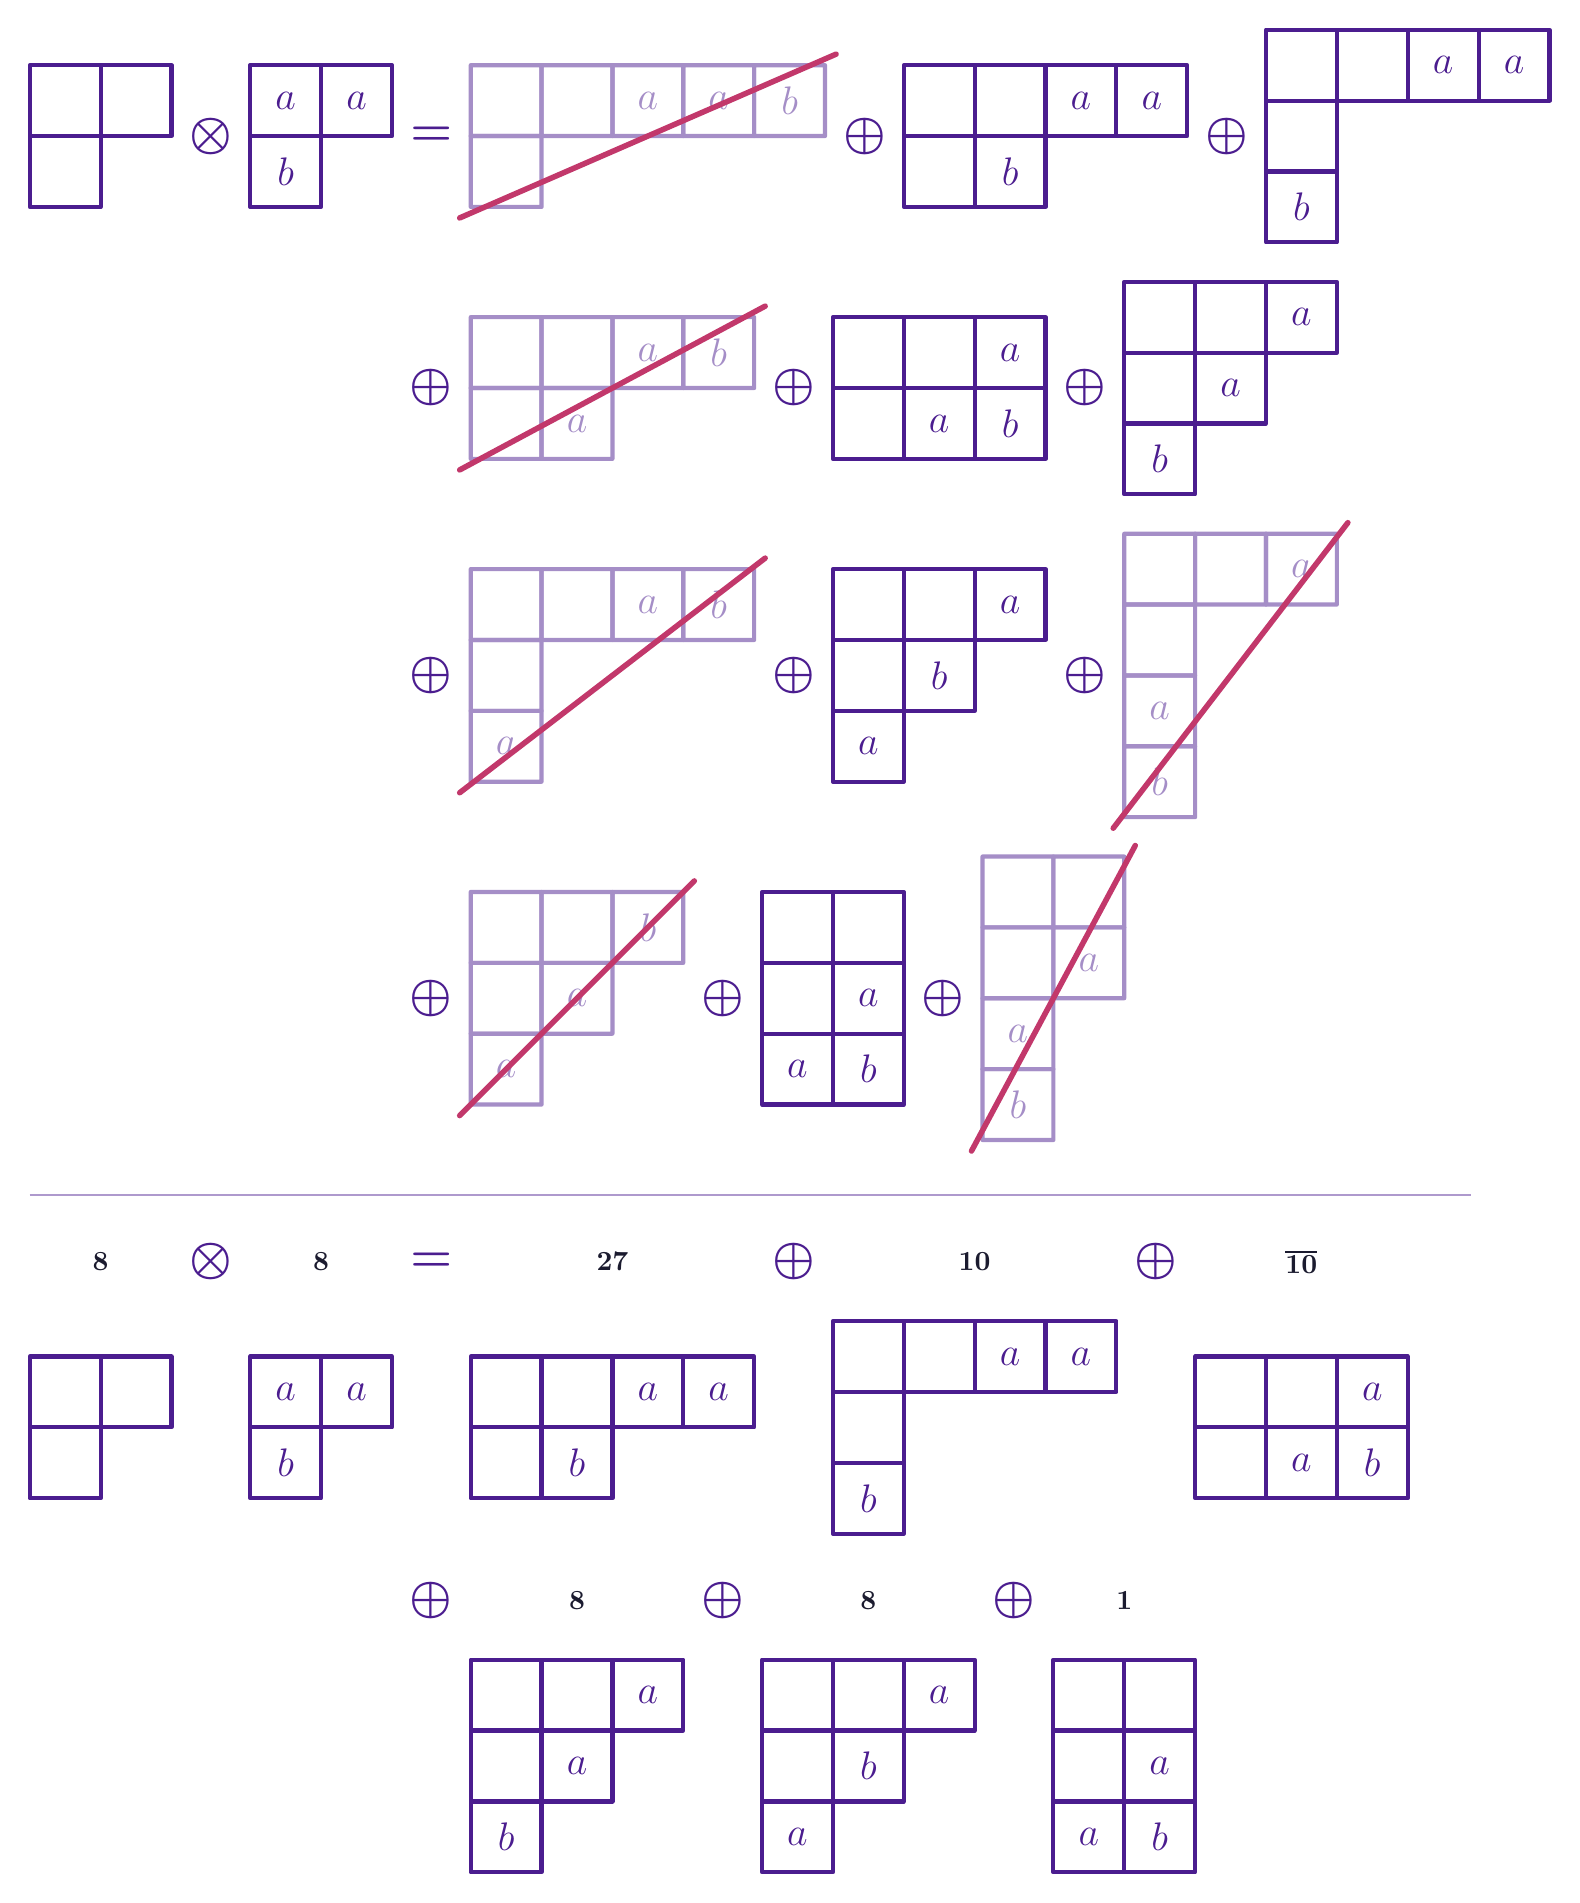
\begin{tikzpicture}[every node/.style={text=ink}]
\draw[P,line width=1.5pt,line join=round] (0.000,0.900) rectangle (0.900,0.000);
\draw[P,line width=1.5pt,line join=round] (0.900,0.900) rectangle (1.800,0.000);
\draw[P,line width=1.5pt,line join=round] (0.000,0.000) rectangle (0.900,-0.900);
\node[text=P] at (2.300,0.000) {\LARGE$\bm{\otimes}$};
\draw[P,line width=1.5pt,line join=round] (2.800,0.900) rectangle (3.700,0.000);
\node[text=P] at (3.250,0.450) {\Large$a$};
\draw[P,line width=1.5pt,line join=round] (3.700,0.900) rectangle (4.600,0.000);
\node[text=P] at (4.150,0.450) {\Large$a$};
\draw[P,line width=1.5pt,line join=round] (2.800,0.000) rectangle (3.700,-0.900);
\node[text=P] at (3.250,-0.450) {\Large$b$};
\node[text=P] at (5.100,0.000) {\LARGE$\bm{=}$};
\begin{scope}[transparency group,opacity=.5]
\draw[P,line width=1.5pt,line join=round] (5.600,0.900) rectangle (6.500,0.000);
\draw[P,line width=1.5pt,line join=round] (6.500,0.900) rectangle (7.400,0.000);
\draw[P,line width=1.5pt,line join=round] (5.600,0.000) rectangle (6.500,-0.900);
\draw[P,line width=1.5pt,line join=round] (7.400,0.900) rectangle (8.300,0.000);
\node[text=P] at (7.850,0.450) {\Large$a$};
\draw[P,line width=1.5pt,line join=round] (8.300,0.900) rectangle (9.200,0.000);
\node[text=P] at (8.750,0.450) {\Large$a$};
\draw[P,line width=1.5pt,line join=round] (9.200,0.900) rectangle (10.100,0.000);
\node[text=P] at (9.650,0.450) {\Large$b$};
\end{scope}
\draw[X,line width=2pt,line cap=round] (5.460,-1.040) -- (10.240,1.040);
\node[text=P] at (10.600,0.000) {\LARGE$\bm{\oplus}$};
\draw[P,line width=1.5pt,line join=round] (11.100,0.900) rectangle (12.000,0.000);
\draw[P,line width=1.5pt,line join=round] (12.000,0.900) rectangle (12.900,0.000);
\draw[P,line width=1.5pt,line join=round] (11.100,0.000) rectangle (12.000,-0.900);
\draw[P,line width=1.5pt,line join=round] (12.900,0.900) rectangle (13.800,0.000);
\node[text=P] at (13.350,0.450) {\Large$a$};
\draw[P,line width=1.5pt,line join=round] (13.800,0.900) rectangle (14.700,0.000);
\node[text=P] at (14.250,0.450) {\Large$a$};
\draw[P,line width=1.5pt,line join=round] (12.000,0.000) rectangle (12.900,-0.900);
\node[text=P] at (12.450,-0.450) {\Large$b$};
\node[text=P] at (15.200,0.000) {\LARGE$\bm{\oplus}$};
\draw[P,line width=1.5pt,line join=round] (15.700,1.350) rectangle (16.600,0.450);
\draw[P,line width=1.5pt,line join=round] (16.600,1.350) rectangle (17.500,0.450);
\draw[P,line width=1.5pt,line join=round] (15.700,0.450) rectangle (16.600,-0.450);
\draw[P,line width=1.5pt,line join=round] (17.500,1.350) rectangle (18.400,0.450);
\node[text=P] at (17.950,0.900) {\Large$a$};
\draw[P,line width=1.5pt,line join=round] (18.400,1.350) rectangle (19.300,0.450);
\node[text=P] at (18.850,0.900) {\Large$a$};
\draw[P,line width=1.5pt,line join=round] (15.700,-0.450) rectangle (16.600,-1.350);
\node[text=P] at (16.150,-0.900) {\Large$b$};
\node[text=P] at (5.100,-3.200) {\LARGE$\bm{\oplus}$};
\begin{scope}[transparency group,opacity=.5]
\draw[P,line width=1.5pt,line join=round] (5.600,-2.300) rectangle (6.500,-3.200);
\draw[P,line width=1.5pt,line join=round] (6.500,-2.300) rectangle (7.400,-3.200);
\draw[P,line width=1.5pt,line join=round] (5.600,-3.200) rectangle (6.500,-4.100);
\draw[P,line width=1.5pt,line join=round] (6.500,-3.200) rectangle (7.400,-4.100);
\node[text=P] at (6.950,-3.650) {\Large$a$};
\draw[P,line width=1.5pt,line join=round] (7.400,-2.300) rectangle (8.300,-3.200);
\node[text=P] at (7.850,-2.750) {\Large$a$};
\draw[P,line width=1.5pt,line join=round] (8.300,-2.300) rectangle (9.200,-3.200);
\node[text=P] at (8.750,-2.750) {\Large$b$};
\end{scope}
\draw[X,line width=2pt,line cap=round] (5.460,-4.240) -- (9.340,-2.160);
\node[text=P] at (9.700,-3.200) {\LARGE$\bm{\oplus}$};
\draw[P,line width=1.5pt,line join=round] (10.200,-2.300) rectangle (11.100,-3.200);
\draw[P,line width=1.5pt,line join=round] (11.100,-2.300) rectangle (12.000,-3.200);
\draw[P,line width=1.5pt,line join=round] (10.200,-3.200) rectangle (11.100,-4.100);
\draw[P,line width=1.5pt,line join=round] (11.100,-3.200) rectangle (12.000,-4.100);
\node[text=P] at (11.550,-3.650) {\Large$a$};
\draw[P,line width=1.5pt,line join=round] (12.000,-2.300) rectangle (12.900,-3.200);
\node[text=P] at (12.450,-2.750) {\Large$a$};
\draw[P,line width=1.5pt,line join=round] (12.000,-3.200) rectangle (12.900,-4.100);
\node[text=P] at (12.450,-3.650) {\Large$b$};
\node[text=P] at (13.400,-3.200) {\LARGE$\bm{\oplus}$};
\draw[P,line width=1.5pt,line join=round] (13.900,-1.850) rectangle (14.800,-2.750);
\draw[P,line width=1.5pt,line join=round] (14.800,-1.850) rectangle (15.700,-2.750);
\draw[P,line width=1.5pt,line join=round] (13.900,-2.750) rectangle (14.800,-3.650);
\draw[P,line width=1.5pt,line join=round] (14.800,-2.750) rectangle (15.700,-3.650);
\node[text=P] at (15.250,-3.200) {\Large$a$};
\draw[P,line width=1.5pt,line join=round] (15.700,-1.850) rectangle (16.600,-2.750);
\node[text=P] at (16.150,-2.300) {\Large$a$};
\draw[P,line width=1.5pt,line join=round] (13.900,-3.650) rectangle (14.800,-4.550);
\node[text=P] at (14.350,-4.100) {\Large$b$};
\node[text=P] at (5.100,-6.850) {\LARGE$\bm{\oplus}$};
\begin{scope}[transparency group,opacity=.5]
\draw[P,line width=1.5pt,line join=round] (5.600,-5.500) rectangle (6.500,-6.400);
\draw[P,line width=1.5pt,line join=round] (6.500,-5.500) rectangle (7.400,-6.400);
\draw[P,line width=1.5pt,line join=round] (5.600,-6.400) rectangle (6.500,-7.300);
\draw[P,line width=1.5pt,line join=round] (5.600,-7.300) rectangle (6.500,-8.200);
\node[text=P] at (6.050,-7.750) {\Large$a$};
\draw[P,line width=1.5pt,line join=round] (7.400,-5.500) rectangle (8.300,-6.400);
\node[text=P] at (7.850,-5.950) {\Large$a$};
\draw[P,line width=1.5pt,line join=round] (8.300,-5.500) rectangle (9.200,-6.400);
\node[text=P] at (8.750,-5.950) {\Large$b$};
\end{scope}
\draw[X,line width=2pt,line cap=round] (5.460,-8.340) -- (9.340,-5.360);
\node[text=P] at (9.700,-6.850) {\LARGE$\bm{\oplus}$};
\draw[P,line width=1.5pt,line join=round] (10.200,-5.500) rectangle (11.100,-6.400);
\draw[P,line width=1.5pt,line join=round] (11.100,-5.500) rectangle (12.000,-6.400);
\draw[P,line width=1.5pt,line join=round] (10.200,-6.400) rectangle (11.100,-7.300);
\draw[P,line width=1.5pt,line join=round] (10.200,-7.300) rectangle (11.100,-8.200);
\node[text=P] at (10.650,-7.750) {\Large$a$};
\draw[P,line width=1.5pt,line join=round] (12.000,-5.500) rectangle (12.900,-6.400);
\node[text=P] at (12.450,-5.950) {\Large$a$};
\draw[P,line width=1.5pt,line join=round] (11.100,-6.400) rectangle (12.000,-7.300);
\node[text=P] at (11.550,-6.850) {\Large$b$};
\node[text=P] at (13.400,-6.850) {\LARGE$\bm{\oplus}$};
\begin{scope}[transparency group,opacity=.5]
\draw[P,line width=1.5pt,line join=round] (13.900,-5.050) rectangle (14.800,-5.950);
\draw[P,line width=1.5pt,line join=round] (14.800,-5.050) rectangle (15.700,-5.950);
\draw[P,line width=1.5pt,line join=round] (13.900,-5.950) rectangle (14.800,-6.850);
\draw[P,line width=1.5pt,line join=round] (13.900,-6.850) rectangle (14.800,-7.750);
\node[text=P] at (14.350,-7.300) {\Large$a$};
\draw[P,line width=1.5pt,line join=round] (15.700,-5.050) rectangle (16.600,-5.950);
\node[text=P] at (16.150,-5.500) {\Large$a$};
\draw[P,line width=1.5pt,line join=round] (13.900,-7.750) rectangle (14.800,-8.650);
\node[text=P] at (14.350,-8.200) {\Large$b$};
\end{scope}
\draw[X,line width=2pt,line cap=round] (13.760,-8.790) -- (16.740,-4.910);
\node[text=P] at (5.100,-10.950) {\LARGE$\bm{\oplus}$};
\begin{scope}[transparency group,opacity=.5]
\draw[P,line width=1.5pt,line join=round] (5.600,-9.600) rectangle (6.500,-10.500);
\draw[P,line width=1.5pt,line join=round] (6.500,-9.600) rectangle (7.400,-10.500);
\draw[P,line width=1.5pt,line join=round] (5.600,-10.500) rectangle (6.500,-11.400);
\draw[P,line width=1.5pt,line join=round] (6.500,-10.500) rectangle (7.400,-11.400);
\node[text=P] at (6.950,-10.950) {\Large$a$};
\draw[P,line width=1.5pt,line join=round] (5.600,-11.400) rectangle (6.500,-12.300);
\node[text=P] at (6.050,-11.850) {\Large$a$};
\draw[P,line width=1.5pt,line join=round] (7.400,-9.600) rectangle (8.300,-10.500);
\node[text=P] at (7.850,-10.050) {\Large$b$};
\end{scope}
\draw[X,line width=2pt,line cap=round] (5.460,-12.440) -- (8.440,-9.460);
\node[text=P] at (8.800,-10.950) {\LARGE$\bm{\oplus}$};
\draw[P,line width=1.5pt,line join=round] (9.300,-9.600) rectangle (10.200,-10.500);
\draw[P,line width=1.5pt,line join=round] (10.200,-9.600) rectangle (11.100,-10.500);
\draw[P,line width=1.5pt,line join=round] (9.300,-10.500) rectangle (10.200,-11.400);
\draw[P,line width=1.5pt,line join=round] (10.200,-10.500) rectangle (11.100,-11.400);
\node[text=P] at (10.650,-10.950) {\Large$a$};
\draw[P,line width=1.5pt,line join=round] (9.300,-11.400) rectangle (10.200,-12.300);
\node[text=P] at (9.750,-11.850) {\Large$a$};
\draw[P,line width=1.5pt,line join=round] (10.200,-11.400) rectangle (11.100,-12.300);
\node[text=P] at (10.650,-11.850) {\Large$b$};
\node[text=P] at (11.600,-10.950) {\LARGE$\bm{\oplus}$};
\begin{scope}[transparency group,opacity=.5]
\draw[P,line width=1.5pt,line join=round] (12.100,-9.150) rectangle (13.000,-10.050);
\draw[P,line width=1.5pt,line join=round] (13.000,-9.150) rectangle (13.900,-10.050);
\draw[P,line width=1.5pt,line join=round] (12.100,-10.050) rectangle (13.000,-10.950);
\draw[P,line width=1.5pt,line join=round] (13.000,-10.050) rectangle (13.900,-10.950);
\node[text=P] at (13.450,-10.500) {\Large$a$};
\draw[P,line width=1.5pt,line join=round] (12.100,-10.950) rectangle (13.000,-11.850);
\node[text=P] at (12.550,-11.400) {\Large$a$};
\draw[P,line width=1.5pt,line join=round] (12.100,-11.850) rectangle (13.000,-12.750);
\node[text=P] at (12.550,-12.300) {\Large$b$};
\end{scope}
\draw[X,line width=2pt,line cap=round] (11.960,-12.890) -- (14.040,-9.010);
\draw[rule,line width=.7pt] (0,-13.450) -- (18.300,-13.450);
\draw[P,line width=1.5pt,line join=round] (0.000,-15.500) rectangle (0.900,-16.400);
\draw[P,line width=1.5pt,line join=round] (0.900,-15.500) rectangle (1.800,-16.400);
\draw[P,line width=1.5pt,line join=round] (0.000,-16.400) rectangle (0.900,-17.300);
\node at (0.900,-14.300) {$\mathbf{8}$};\node[text=P] at (2.300,-14.300) {\LARGE$\bm{\otimes}$};
\draw[P,line width=1.5pt,line join=round] (2.800,-15.500) rectangle (3.700,-16.400);
\node[text=P] at (3.250,-15.950) {\Large$a$};
\draw[P,line width=1.5pt,line join=round] (3.700,-15.500) rectangle (4.600,-16.400);
\node[text=P] at (4.150,-15.950) {\Large$a$};
\draw[P,line width=1.5pt,line join=round] (2.800,-16.400) rectangle (3.700,-17.300);
\node[text=P] at (3.250,-16.850) {\Large$b$};
\node at (3.700,-14.300) {$\mathbf{8}$};\node[text=P] at (5.100,-14.300) {\LARGE$\bm{=}$};
\node at (7.400,-14.300) {$\mathbf{27}$};
\draw[P,line width=1.5pt,line join=round] (5.600,-15.500) rectangle (6.500,-16.400);
\draw[P,line width=1.5pt,line join=round] (6.500,-15.500) rectangle (7.400,-16.400);
\draw[P,line width=1.5pt,line join=round] (5.600,-16.400) rectangle (6.500,-17.300);
\draw[P,line width=1.5pt,line join=round] (7.400,-15.500) rectangle (8.300,-16.400);
\node[text=P] at (7.850,-15.950) {\Large$a$};
\draw[P,line width=1.5pt,line join=round] (8.300,-15.500) rectangle (9.200,-16.400);
\node[text=P] at (8.750,-15.950) {\Large$a$};
\draw[P,line width=1.5pt,line join=round] (6.500,-16.400) rectangle (7.400,-17.300);
\node[text=P] at (6.950,-16.850) {\Large$b$};
\node[text=P] at (9.700,-14.300) {\LARGE$\bm{\oplus}$};
\node at (12.000,-14.300) {$\mathbf{10}$};
\draw[P,line width=1.5pt,line join=round] (10.200,-15.050) rectangle (11.100,-15.950);
\draw[P,line width=1.5pt,line join=round] (11.100,-15.050) rectangle (12.000,-15.950);
\draw[P,line width=1.5pt,line join=round] (10.200,-15.950) rectangle (11.100,-16.850);
\draw[P,line width=1.5pt,line join=round] (12.000,-15.050) rectangle (12.900,-15.950);
\node[text=P] at (12.450,-15.500) {\Large$a$};
\draw[P,line width=1.5pt,line join=round] (12.900,-15.050) rectangle (13.800,-15.950);
\node[text=P] at (13.350,-15.500) {\Large$a$};
\draw[P,line width=1.5pt,line join=round] (10.200,-16.850) rectangle (11.100,-17.750);
\node[text=P] at (10.650,-17.300) {\Large$b$};
\node[text=P] at (14.300,-14.300) {\LARGE$\bm{\oplus}$};
\node at (16.150,-14.300) {$\overline{\mathbf{10}}$};
\draw[P,line width=1.5pt,line join=round] (14.800,-15.500) rectangle (15.700,-16.400);
\draw[P,line width=1.5pt,line join=round] (15.700,-15.500) rectangle (16.600,-16.400);
\draw[P,line width=1.5pt,line join=round] (14.800,-16.400) rectangle (15.700,-17.300);
\draw[P,line width=1.5pt,line join=round] (15.700,-16.400) rectangle (16.600,-17.300);
\node[text=P] at (16.150,-16.850) {\Large$a$};
\draw[P,line width=1.5pt,line join=round] (16.600,-15.500) rectangle (17.500,-16.400);
\node[text=P] at (17.050,-15.950) {\Large$a$};
\draw[P,line width=1.5pt,line join=round] (16.600,-16.400) rectangle (17.500,-17.300);
\node[text=P] at (17.050,-16.850) {\Large$b$};
\node[text=P] at (5.100,-18.600) {\LARGE$\bm{\oplus}$};
\node at (6.950,-18.600) {$\mathbf{8}$};
\draw[P,line width=1.5pt,line join=round] (5.600,-19.350) rectangle (6.500,-20.250);
\draw[P,line width=1.5pt,line join=round] (6.500,-19.350) rectangle (7.400,-20.250);
\draw[P,line width=1.5pt,line join=round] (5.600,-20.250) rectangle (6.500,-21.150);
\draw[P,line width=1.5pt,line join=round] (6.500,-20.250) rectangle (7.400,-21.150);
\node[text=P] at (6.950,-20.700) {\Large$a$};
\draw[P,line width=1.5pt,line join=round] (7.400,-19.350) rectangle (8.300,-20.250);
\node[text=P] at (7.850,-19.800) {\Large$a$};
\draw[P,line width=1.5pt,line join=round] (5.600,-21.150) rectangle (6.500,-22.050);
\node[text=P] at (6.050,-21.600) {\Large$b$};
\node[text=P] at (8.800,-18.600) {\LARGE$\bm{\oplus}$};
\node at (10.650,-18.600) {$\mathbf{8}$};
\draw[P,line width=1.5pt,line join=round] (9.300,-19.350) rectangle (10.200,-20.250);
\draw[P,line width=1.5pt,line join=round] (10.200,-19.350) rectangle (11.100,-20.250);
\draw[P,line width=1.5pt,line join=round] (9.300,-20.250) rectangle (10.200,-21.150);
\draw[P,line width=1.5pt,line join=round] (9.300,-21.150) rectangle (10.200,-22.050);
\node[text=P] at (9.750,-21.600) {\Large$a$};
\draw[P,line width=1.5pt,line join=round] (11.100,-19.350) rectangle (12.000,-20.250);
\node[text=P] at (11.550,-19.800) {\Large$a$};
\draw[P,line width=1.5pt,line join=round] (10.200,-20.250) rectangle (11.100,-21.150);
\node[text=P] at (10.650,-20.700) {\Large$b$};
\node[text=P] at (12.500,-18.600) {\LARGE$\bm{\oplus}$};
\node at (13.900,-18.600) {$\mathbf{1}$};
\draw[P,line width=1.5pt,line join=round] (13.000,-19.350) rectangle (13.900,-20.250);
\draw[P,line width=1.5pt,line join=round] (13.900,-19.350) rectangle (14.800,-20.250);
\draw[P,line width=1.5pt,line join=round] (13.000,-20.250) rectangle (13.900,-21.150);
\draw[P,line width=1.5pt,line join=round] (13.900,-20.250) rectangle (14.800,-21.150);
\node[text=P] at (14.350,-20.700) {\Large$a$};
\draw[P,line width=1.5pt,line join=round] (13.000,-21.150) rectangle (13.900,-22.050);
\node[text=P] at (13.450,-21.600) {\Large$a$};
\draw[P,line width=1.5pt,line join=round] (13.900,-21.150) rectangle (14.800,-22.050);
\node[text=P] at (14.350,-21.600) {\Large$b$};
\end{tikzpicture}
\end{document}
